\documentclass{oci}
\usepackage[utf8]{inputenc}
\usepackage{lipsum}
\usepackage{tikz}
\usepackage{amsmath}

% \definecolor{color1}{HTML}{D81B60}
% \definecolor{color2}{HTML}{1E88E5}
% \definecolor{color3}{HTML}{FFC107}
\definecolor{color1}{HTML}{648FFF}
\definecolor{color2}{HTML}{DC267F}
\definecolor{color3}{HTML}{FFB000}

\title{Viaje a la playa}

\begin{document}
\begin{problemDescription}
David está organizando un viaje a la playa con sus amigos.
%
Su ciudad puede ser representada por una grilla de $n$ filas y $m$ columnas.
%
Para referirnos a la celda en la fila $i$-ésima y columna $j$-ésima usaremos
el par $(i,j)$.
%
David comienza su viaje en la esquina superior izquierda $(1, 1)$ y debe
moverse por la grilla siguiendo un \emph{camino} hasta alcanzar la esquina
inferior derecha $(n, m)$.
%
En un movimiento, David puede pasar de la celda actual a una celda contigua
que comparta un lado.
%
El largo del camino se define como la cantidad de movimientos.

Adicionalmente, cada celda tiene un color asociado.
%
El color de cada celda es representado por un número $C_{(i,j)}$ que va entre $1$ y $k$.
%
David le prometió a sus amigos buscar un camino \emph{agradable}.
%
Para que un camino sea agradable ningún par de celdas consecutivas
puede tener el mismo color.
%
Es decir, si en algún momento el camino pasa de la celda $(i_1,j_1)$ a la
celda $(i_2,j_2)$ este solo puede ser agradable si $C_{(i_1,j_1)} \neq C_{(i_2,j_2)}$.

% Por ejemplo, un mapa posible con $n = 3$, $m = 3$ y $k = 3$ es:
% \begin{gather*}
% 1\ 2\ 1\\
% 3\ 3\ 2\\
% 3\ 3\ 1
% \end{gather*}
Por ejemplo, las siguientes figuras representan un posible mapa de la ciudad para
una grilla con $n=3$, $m=3$ y $k=3$.
%
El número en cada celda corresponde a su color.
\begin{figure}[!h]
\centering
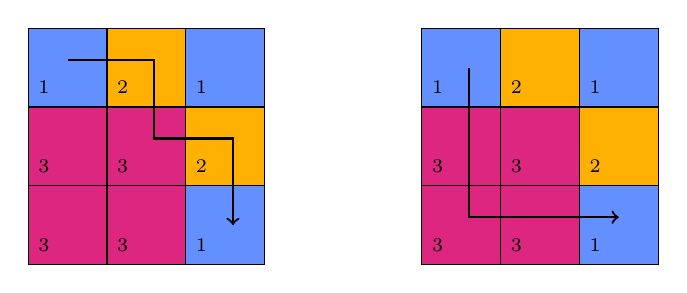
\begin{tikzpicture}
\fill[color1,draw=black] (0,0) rectangle (1,1); \fill[color3,draw=black] (1,0) rectangle (2,1); \fill[color1,draw=black] (2,0) rectangle (3,1);
\fill[color2,draw=black] (0,0) rectangle (1,-1); \fill[color2,draw=black] (1,0) rectangle (2,-1); \fill[color3,draw=black] (2,0) rectangle (3,-1);
\fill[color2,draw=black] (0,-2) rectangle (1,-1); \fill[color2,draw=black] (1,-2) rectangle (2,-1); \fill[color1,draw=black] (2,-2) rectangle (3,-1);
\node at (0.2, 0.25) {\scriptsize 1}; \node at (1.2, 0.25) {\scriptsize 2}; \node at (2.2, 0.25) {\scriptsize 1};
\node at (0.2, -.75) {\scriptsize 3}; \node at (1.2, -.75) {\scriptsize 3}; \node at (2.2, -.75) {\scriptsize 2};
\node at (0.2, -1.75) {\scriptsize 3}; \node at (1.2, -1.75) {\scriptsize 3}; \node at (2.2, -1.75) {\scriptsize 1};
% \draw[thick,->] (0.5,0.6) -- (2.6,0.6) -- (2.6,-1.5);
\draw[thick,->] (0.5,0.6) -- (1.6,0.6) -- (1.6, -.4) -- (2.6, -.4) -- (2.6,-1.5);

\fill[color1,draw=black] (5,0) rectangle (6,1); \fill[color3,draw=black] (6,0) rectangle (7,1); \fill[color1,draw=black] (7,0) rectangle (8,1);
\fill[color2,draw=black] (5,0) rectangle (6,-1); \fill[color2,draw=black] (6,0) rectangle (7,-1); \fill[color3,draw=black] (7,0) rectangle (8,-1);
\fill[color2,draw=black] (5,-2) rectangle (6,-1); \fill[color2,draw=black] (6,-2) rectangle (7,-1); \fill[color1,draw=black] (7,-2) rectangle (8,-1);
\node at (5.2, 0.25) {\scriptsize 1}; \node at (6.2, 0.25) {\scriptsize 2}; \node at (7.2, 0.25) {\scriptsize 1};
\node at (5.2, -.75) {\scriptsize 3}; \node at (6.2, -.75) {\scriptsize 3}; \node at (7.2, -.75) {\scriptsize 2};
\node at (5.2, -1.75) {\scriptsize 3}; \node at (6.2, -1.75) {\scriptsize 3}; \node at (7.2, -1.75) {\scriptsize 1};
\draw[thick,->] (5.6,0.5) -- (5.6,-1.4) -- (7.5,-1.4);
\end{tikzpicture}
\end{figure}

Cada figura muestra con una flecha un camino que va desde $(1,1)$ hasta $(3,3)$.
%
El camino en la figura de la izquierda es agradable pues nunca atraviesa dos celdas
consecutivas con el mismo color.
%
El camino de la derecha no es agradable, ya que la segunda, tercera y cuarta
celda son del mismo color.
%
El largo del camino en ambos casos es $4$.

David observa el mapa muy confundido sin poder encontrar un camino agradable y necesita de tu
ayuda.
%
Dada la descripción de la grilla, tu tarea es determinar si existe un camino agradable
y, si existe, imprimir la distancia del camino agradable más corto.

\end{problemDescription}


\begin{inputDescription}
La primera línea contiene tres enteros $n, m$ y $k$
($1 \leq n, m \leq 1000$, $2 \leq n\times m \leq 10^5$ y $2 \leq k \leq n \times m$)
que corresponden a las dimensiones de la ciudad y la cantidad de colores que hay.

A continuación siguen $n$ líneas, cada una con $m$ enteros que van entre $1$ y $k$.
%
El $j$-ésimo entero de la $i$-ésima línea representa a $C_{(i,j)}$, el color de la celda $(i,j)$.

\end{inputDescription}

\begin{outputDescription}
  La salida debe contener el largo del camino agradable más corto entre la celda (1, 1)
  y la celda $(n, m)$.
  %
  Si este camino no existe debes imprimir -1.

\end{outputDescription}

\begin{scoreDescription}
  \subtask{20}
  Se probaran varios casos en que $n = 1$, es decir, el mapa es solo una fila.
  \subtask{20}
  Se probaran varios casos en que $n = 2$ y $k = 2$, es decir, son dos filas con solo dos colores.
  \subtask{20}
  Se probaran varios casos en que $n = 2$.
  \subtask{40}
  Se probaran varios casos sin más restricciones.
\end{scoreDescription}

\begin{sampleDescription}
\sampleIO{sample-1}
\sampleIO{sample-2}
\end{sampleDescription}

\end{document}
